\title{Collision Avoidance of an Autonomous Quadrotor in Low-Altitude Heterogeneous Flights}

\documentclass[journal,11pt,onecolumn,draftclsnofoot,]{IEEEtran}

\usepackage[noadjust]{cite}

% \usepackage{natbib}

\usepackage[left=1.25in,right=1.25in,top=1in,bottom=1in]{geometry}

\usepackage{amsmath}

\usepackage{color}

\usepackage[pdftex]{graphicx}

%\usepackage{caption}

\usepackage{subcaption}

\usepackage{array}

\usepackage{multicol}

\usepackage{url}

\graphicspath{{./figure/}}

\ifCLASSOPTIONcompsoc
 \usepackage[caption=false,font=normalsize,labelfont=sf,textfont=sf]{subfig}
\else
 \usepackage[caption=false,font=footnotesize]{subfig}
\fi

\begin{document}
\title{Collision Avoidance of an Autonomous Quadrotor in Low-Altitude Heterogeneous Flights}

\author{Zhilong Liu, Aislan G. Foina, Karl Hedrick, Raja Sengupta}

% Header
%\markboth{Header Here}
%{Shell \MakeLowercase{\textit{et al.}}: Bare Demo of IEEEtran.cls for Journals}

% show title
\maketitle
\pagenumbering{gobble}

\begin{abstract}
Automatic dependent surveillance-broadcast (ADS-B) is regarded as a promising solution to the Sense and Avoid (SAA) problem for small Unmanned Aircraft Systems (sUAS), especially for high speed flights where long-range sensing is not possible. In this paper, a hybrid controller with ADS-B is introduced to enable a small quadrotor to perform optimal collision avoidance with a high-speed helicopter during autonomous navigation. First, a position controller and a safety controller are formulated independently. Then, they are combined together to form a hybrid automaton where transitions between the controllers are performed. Simulation shows the effectiveness of the hybrid controller.
\end{abstract}

% keywords
\begin{IEEEkeywords}
sliding mode, optimal control, collision avoidance, quadrotor.
\end{IEEEkeywords}

% \IEEEpeerreviewmaketitle

\section{\textbf{Introduction}}

Recent advances in sensing and computing technology has made unmanned aerial vehicles/systems (UAV/UAS) low-cost but still increasingly capable of executing complex missions in challenging environments. Among all types of UAVs, quadrotor helicopters have become increasingly popular for several reasons. Unlike a conventional fixed-wing UAV, a quadrotor has hovering capability and omni-directional maneuverability, although the additional motors make it not as power-efficient. They have gained popularity in a vast range of civilian applications, including search and rescue, disaster relief, agricultural imaging, and filming. In response, the Federal Aviation Administration (FAA) has issued the Notice of Proposed Rulemaking (NPRM) on UAS certifications \cite{faa-nprm}, indicating that a large number of UAS will present in the National Airspace System (NAS) in the near future. However, since UAS are inherently different from manned aircraft, the integration will face many challenges. Collision avoidance between manned and unmanned aircraft is a good example. This is especially true for low-altitude flights, where a heterogeneous mix of manned and unmanned aircraft could present in close proximity simultaneously. To ensure safety, a reliable collision avoidance system must be deployed in a large scale.

In general, there are two types of collision avoidance mechanisms, namely cooperative avoidance and non-cooperative avoidance. Non-cooperative avoidance relies on remote sensing technologies, such as radars, laser range finders, and cameras, to detect obstacles. Aircraft with these sensors could detect a wide range of obstacles. However, for sUAS with limited payload capacity, the detection range is limited, which causes safety concern when vehicles are traveling at very high speeds. On the other hand, cooperative avoidance relies on long-range communication between aircraft. A good example is aircraft equipping with Automatic Dependent Surveillance-Broadcast (ADS-B). Aircraft with (ADS-B)-In technology could obtain traffic information of nearby aircraft with (ADS-B)-Out. The communication link is critical in this type of avoidance, and obstacles that are not in the communication network are not detected.

To solve the collision avoidance problem, the FAA has mandated that aircraft flying in the US must be equipped with (ADS-B)-Out by 2020. As a result, ADS-B technology is growing rapidly in recent years. ADS-B is a transponder broadcasting mainly the GPS-based traffic data of the own aircraft, which could be received in real-time by the aircraft nearby. The broadcasting frequency is 1 Hz. To address the UAS integration problem, manufacturers start producing small-size ADS-B transponders specifically for small UAS. Examples are XPG-TR from Sagetech \cite{sagetech} and ADS-B ONE from NextGen UAS Transponders \cite{ads-b-one}. Although there are many alternative avoidance sensing technologies available, they are not likely to replace ADS-B. Therefore, in this paper, we are mainly concerned with cooperative avoidance with ADS-B.

Given the collision detection mechanism, what remains is a hybrid controller with both position and safety control capability, which constitute the contribution of this paper. The position controller is a set of concisely formulated sliding mode controllers augmented with dynamic surface control techniques. The safety controller generates a horizontal optimal control action that minimizes the reaction time needed to avoid collision.

In this paper, we want to address the following scenario: A manned helicopter ambulance equipped with (ADS-B)-Out is flying at a low altitude to pick up a patient, when a quadrotor UAV with (ADS-B)-In is delivering packages autonomously. The quadrotor can receive real-time traffic information of the helicopter. If collision is possible, the quadrotor would avoid the manned helicopter. The avoidance maneuver is performed exclusively by the quadrotor UAV.

\section{\textbf{Literature Review}}

\subsection{Position Controller}
Since a quadrotor uses only four inputs to control six degrees of freedom (DOF), it is an underactuated system. Specifically, the horizontal movements are highly coupled with the roll and pitch angles. Despite of the nonlinear nature of a quadrotors, linear controllers such as PID and LQ can still be applied. One simple stabilizing strategy is to use four PID controllers to control altitude and Euler angles \cite{bouabdallah2004pid}. If position tracking is required, two additional PID controllers coupling with roll and pitch are needed \cite{li2011dynamic}. However, since the system is highly nonlinear, tuning six PID controllers simultaneously is non-trivial to achieve good performance. From \cite{bouabdallah2004pid}, LQ controllers give no better performance than PID. Therefore, more insightful nonlinear controllers are preferred.

Many researchers have tried a variety of nonlinear control methods to stabilize a quadrotor. A majority of these efforts focus on stabilizing the altitude and Euler angles \cite{bouabdallah2005backstepping, bouchoucha2008step, bouadi2011adaptive}. Furthermore, to enable horizontal position tracking, one has to either use backstepping \cite{lee2009feedback,madani2006backstepping,bouadi2007sliding,huang2010adaptive} or augment the dynamics with control inputs as additional states \cite{lee2009feedback}. However, both approaches could only be used for highly simplified dynamics [\citen{bouabdallah2005backstepping}, \citen{lee2009feedback}] because they require taking the fourth time derivative of the state equations, which leads to explosion of terms in the control laws. In fact, it is practically impossible to derive a position controller using backstepping and dynamic input augmentation from a full quadrotor dynamic model. To avoid the explosion of terms, a new set of sliding mode controllers complemented with dynamic surface control (DSC) filters \cite{song2011dynamic} were developed in this paper. The resulted control laws can accurately represent the full quadrotor dynamic model with minimal simplification, while keeping the equations concise and manageable. The stability proof of DSC using Lyapunov's second method is given in \cite{song2011dynamic}. In the following, we will simply apply the approach.

\subsection{Avoidance Controller}

Aircraft collision avoidance has a rich history in the literature, and is generally referred to as the free-flight problem. Given the ADS-B position data, many avoidance algorithms could be implemented. Typically, the aircraft is modeled as point mass with a constant velocity. A collision avoidance algorithm based on geometric approach is presented in \cite{park2008uav}. The collision detection is achieved by comparing a miss distance vector with a pre-specified minimum separation distance. The control commands are bank and pitch angles, both are defined as functions of some time constants. However, the lack of velocity feedback determines that the minimum separation distance must be specified conservatively, and thus it is not an optimal avoidance strategy.

If sensor noise is taken into account, a probabilistic algorithm is described in \cite{kim2007uav}, where the maneuvers are a function of predefined threat levels generated from Monte Carlo simulations. The probabilistic trajectory models of the own UAV are Gaussian, and models of the intruder UAV are exponential. But again, this model is lack of any sense of optimality.

The first attempt on addressing the collision avoidance problem in an optimal manner is presented in \cite{schouwenaars2001mixed, mellinger2012mixed}. The avoidance problem is formulated as a path planning problem, in which the optimal path could be found by solving a mixed integer programming problem. The forbidden zone is set to be rectangular constraints for simplicity. This method can be easily extended to handle multi-vehicle scenarios with stationary and moving obstacles. However, the number of constraints increase exponentially with the number of vehicles and obstacles. The intensive computation only allows sub-optimal solutions in real-time applications.

In \cite{krozel1996free} and \cite{hoffmann2008decentralized}, the cooperative free flight avoidance is formulated as an optimal control problem in 2D relative frames for fixed wing aircraft and quadrotors, respectively. In \cite{hoffmann2008decentralized}, the optimal control is defined as the maximum acceleration with a constant optimal heading. Consequently, a real-time avoid set can be computed. The derived heading is optimal because the reaction time need to perform the avoidance maneuver is minimal, and the minimum separation is barely achieved when the two vehicles are closest to each other. However, the safety set computation is also expensive. 

To avoid the computation problem, we need to limit the number of vehicles and model complexity. The number of vehicle could be minimized by establishing an air highway system \cite{chen2015safe}. The safety controller in \cite{hoffmann2008decentralized} is derived from a simplified two-dimensional model. Once the controller is applied to a full 3D dynamic model, the optimality is not longer guaranteed strictly for two reasons. First, a quadrotor has rotational inertia, so the maximum acceleration could not be obtained instantaneously. Furthermore, aerodynamic drag at high velocity also reduce the maximum acceleration available. Although the model difference is almost negligible in the low-acceleration drone-drone avoidance case ($\sim 1.5m/s^2$), it is not valid anymore for heterogeneous avoidance, because the maximum acceleration is pushed further  ($\sim 10m/s^2$) in high-speed scenarios. In this paper, we apply a similar safety controller to the quadrotor, with minor modifications, to ensure avoidance optimality.

\section{\textbf{Dynamic Model}} \label{sec:dynamic_model}

The dynamic model of a quadrotor is similar to a typical airplane with a different set of forces. Define a fixed inertial world frame $\mathcal{W}$ and a non-inertial body frame $\mathcal{B}$ attached to the center of gravity of the quadrotor (Figure \ref{fig:frames}). The following is a list of variables used to describe the dynamics of a quadrotor.

\begin{itemize}
\item $\boldsymbol{X}=[X\; Y\; Z]^T$: quadrotor position in $\mathcal{W}$;
\item $\boldsymbol{x}=[x\; y\; z]^T$: quadrotor position in $\mathcal{B}$;
\item $\boldsymbol{V}=[V_X\; V_Y\; V_Z]^T$: quadrotor velocity in $\mathcal{W}$;
\item $\boldsymbol{\Theta}=[\phi\; \theta\; \psi]^T$: Euler angles roll, pitch, and yaw in $\mathcal{B}$;
\item $\boldsymbol{\omega}=[\omega _x\; \omega _y\; \omega _z]^T$: quadrotor angular velocity in $\mathcal{B}$;
\item $\boldsymbol{I}=diag(I_x,I_y,I_z)$: mass moment of inertia in $\mathcal{B}$;
\item $\omega _{r_i}$: motor speeds, $i=1,2,3,4$;
\item $\Omega=-\omega _{r_1}+\omega _{r_2}-\omega _{r_3}+\omega _{r_4}$: sum of motor speeds;
\item $k_f, k_m$: motor thrust and torque coefficients, respectively;
\item $c_t, c_r$: translational and rotational friction coefficients, respectively;
\item $l$: moment arm from the origin of $\mathcal{B}$ to each motor.
\end{itemize}

The free-body diagram of a quadrotor is shown in Figure \ref{fig:FBD}. Each motor produces a thrust $T_{r_i}$ and a torque $\tau _{r_i}$, with $i=1,2,3,4$. It is common to assume that the motor forces are proportional to the angular speed squared $\omega _{r_i}^2$, and the control inputs $\boldsymbol{U}$ satisfies the following linear transformation, with appropriate constraints (\ref{eq:controls}).

\begin{figure}
    \centering
    \begin{subfigure}[b]{.45\columnwidth}
        \centering
        \includegraphics[width=\columnwidth]{frames_quadrotor}
        \caption{The reference frames of a quadrotor.}
        \label{fig:frames}
    \end{subfigure}%
	\hfill
    \begin{subfigure}[b]{.45\columnwidth}
        \centering
        \includegraphics[width=\columnwidth]{FBD_quadrotor}
        \caption{The free-body diagram of a quadrotor.}
        \label{fig:FBD}
    \end{subfigure}
    \caption{Formulation of the quadrotor model}
    \label{fig:formulation_quadrotor}
\end{figure}

\begin{equation}
\label{eq:controls}
\begin{split}
\begin{matrix}
\begin{matrix}
\boldsymbol{U}=
\begin{bmatrix}
U_1\\ U_2\\ U_3\\ U_4
\end{bmatrix}
=
\begin{bmatrix}
k_f & k_f & k_f & k_f\\ 
0 & k_f & 0 & -k_f\\ 
k_f & 0 & -k_f & 0\\ 
k_m & -k_m & k_m & -k_m
\end{bmatrix}
\begin{bmatrix}
\omega _{r_1}^2\\ 
\omega _{r_2}^2\\ 
\omega _{r_3}^2\\ 
\omega _{r_4}^2
\end{bmatrix}\\
\end{matrix}
& \;\;\;\;
\begin{matrix}
0 &< U_1 \le 4 k_f \omega_{r,max}^2 \\
-k_f \omega_{r,max}^2 &\le U_2 \le k_f \omega_{r,max}^2 \\
-k_f \omega_{r,max}^2 &\le U_3 \le k_f \omega_{r,max}^2 \\
-2 k_m \omega_{r,max}^2 &\le U_4 \le 2 k_m \omega_{r,max}^2 \\
\end{matrix}
\end{matrix}
\end{split}
\end{equation}

The control inputs $U_1, U_2l, U_3l, U_4$ represent the total thrust in the $z$ direction and the total motor torques along the roll, pitch, and yaw axes, respectively. These are the control inputs for altitude and Euler angles.
Lastly, we have disturbances from translational drag $c_t \boldsymbol{V}$ and rotational friction $c_r \boldsymbol{\omega}^2$. The state-space equations could be written compactly as (\ref{eq:state-space_compact}):

%\begingroup\makeatletter\def\f@size{11}\check@mathfonts
\begin{equation}
\label{eq:state-space_compact}
\begin{split}
\boldsymbol{\dot{X}}&=\boldsymbol{V} \\
\boldsymbol{\dot{\Theta}}&=R_v^{-1}\boldsymbol{\omega} \\
\boldsymbol{\dot{V}}&=\boldsymbol{g}+\frac{1}{m}\left(-c_t\boldsymbol{V}+R_{\mathcal{B}\rightarrow \mathcal{W}}
\begin{bmatrix}
0\\ 0\\ U_1
\end{bmatrix}
\right) \\
\boldsymbol{\dot{\omega}}&=I^{-1} \left(\boldsymbol{\omega}\times \left(I\boldsymbol{\omega}\right)-\boldsymbol{\omega} \times \left(I_r 
\begin{bmatrix}
0\\ 0\\ \Omega
\end{bmatrix}
\right)-c_r \boldsymbol{\omega}^2+ 
\begin{bmatrix}
U_2l \\ U_3l \\ U_4
\end{bmatrix}
\right)
\end{split}
\end{equation}
%\endgroup

where $R_{\mathcal{B}\rightarrow \mathcal{W}}$ is the rotation matrix from $\mathcal{B}$ to $\mathcal{W}$, and $R_v$ is a linear transformation from $\boldsymbol{\dot{\Theta}}$ to $\boldsymbol{\omega}$. For details of the matrices, refer to \cite{huang2010adaptive}.

%
%\begin{equation*}
%\begin{split}
%R_{\mathcal{B}\rightarrow \mathcal{W}} = &
%\begin{bmatrix}
%c\theta c\psi & s\phi s\theta c\psi - c\phi s\psi & c\phi s\theta c\psi + s\phi s\psi\\ 
%c\theta s\psi & s\phi s\theta s\psi + c\phi c\psi & c\phi s\theta s\psi - s\phi c\psi\\ 
%-s\theta & s\phi c\theta & c\phi c\theta
%\end{bmatrix} \\
%R_v = &
%\begin{bmatrix}
%1 & 0 & -s\theta\\ 
%0 & c\phi & s\phi c\theta\\ 
%0 & -s\phi & c\phi c\theta
%\end{bmatrix}
%\end{split}
%\end{equation*}
%
%The expanded version of the state-space equation is given in equation (\ref{eq:state-space_expanded}) at the end of the paper.

\section{\textbf{Position Controller}}

Given the quadrotor model in Section \ref{sec:dynamic_model}, by following the standard procedure of designing sliding mode controllers, four independent control laws governing the altitude and Euler angles could be derived. However, to achieve horizontal position control, we need two more control laws to relate $X$ and $Y$ to roll ($\phi$) and pitch ($\theta$). And as mentioned before, methods such as backstepping and state augmentation lead to explosion of terms. To avoid that, we applied dynamic surface control (DSC) techniques. In addition, to avoid instability in roll and pitch due to large position errors, a path planner is needed. 

\subsection{\textbf{Sliding Mode Controllers with DSC Filters}} \label{sliding_controller}

Denote the subscript $_d$ to represent the desired value of the variable, we can define the tracking errors to be

\begingroup\makeatletter\def\f@size{10}\check@mathfonts
\begin{equation*}
\begin{split}
\begin{matrix}
e_X \buildrel\triangle\over = X-X_d  & e_\theta \buildrel\triangle\over = \theta - \theta_d \\
e_Y \buildrel\triangle\over = Y-Y_d & e_\phi \buildrel\triangle\over = \phi - \phi_d  \\
e_Z \buildrel\triangle\over = Z-Z_d & e_\psi \buildrel\triangle\over = \psi-\psi_d \\
\end{matrix}
\end{split}
\end{equation*}
\endgroup

where $\phi$ and $\theta$ are the pitch and roll angles required to track $X$ and $Y$. The desired roll $\phi_d$ and pitch $\theta_d$ are tracking $\phi$ and $\theta$ with phase lag defined by time constants $\tau _\phi$ and $\tau _\theta$, respectively. To apply DSC techniques, define two dynamic surface filters to be

\begingroup\makeatletter\def\f@size{10}\check@mathfonts
\begin{equation}
\label{eq:1st-order-filters}
\begin{split}
\tau _\theta \dot{\theta}_d+\theta_d \buildrel\triangle\over = \theta \\
\tau _\phi \dot{\phi}_d+\phi_d \buildrel\triangle\over = \phi \\
\end{split}
\end{equation}
\endgroup

Then, we can define the sliding surfaces to be some desired first-order linear dynamics with tuning parameters $\lambda's$ 

\begingroup\makeatletter\def\f@size{10}\check@mathfonts
\begin{equation*}
\begin{split}
\begin{matrix}
S_X \buildrel\triangle\over = \dot{e}_X + \lambda_X e_X & S_\theta \buildrel\triangle\over = \dot{\theta} + \lambda_\theta e_\theta \\
S_Y \buildrel\triangle\over = \dot{e}_Y + \lambda_Y e_Y & S_\phi \buildrel\triangle\over = \dot{\phi} + \lambda_\phi e_\phi \\
S_Z \buildrel\triangle\over = \dot{e}_Z + \lambda_Z e_Z & S_\psi \buildrel\triangle\over = \dot{e}_\psi + \lambda_\psi e_\psi \\
\end{matrix}
\end{split}
\end{equation*}
\endgroup

Note that the sliding surfaces for $\phi$ and $\theta$ are different from the rest. Take the first time derivatives of the sliding surfaces, and set them equal to the corresponding robustness terms with parameters $\eta's$.

\begingroup\makeatletter\def\f@size{10}\check@mathfonts
\begin{equation}
\label{eq:sliding_surfaces}
\begin{split}
\begin{matrix}
\dot{S}_X \buildrel\triangle\over =-\eta_X sgn S_X & \dot{S}_\theta \buildrel\triangle\over = -\eta_\theta sgn S_\theta \\
\dot{S}_Y \buildrel\triangle\over =-\eta_Y sgn S_Y & \dot{S}_\phi \buildrel\triangle\over = -\eta_\phi sgn S_\phi \\
\dot{S}_Z \buildrel\triangle\over =-\eta_Z sgn S_Z & \dot{S}_\psi \buildrel\triangle\over =-\eta_\psi sgn S_\psi \\
\end{matrix}
\end{split}
\end{equation}
\endgroup

Lastly, substitute (\ref{eq:state-space_compact}) into (\ref{eq:sliding_surfaces}) gives the four control inputs (\ref{eq:U_SM}).

\begingroup\makeatletter\def\f@size{9}\check@mathfonts
\begin{equation}
\label{eq:U_SM}
\begin{split}
U_1 &=  \frac{m}{c\phi c\theta} \left[ \left( -g+\frac{c_t}{m}V_Z \right) + \left(\ddot{Z}_d - \lambda_Z \dot{e}_Z \right) - \eta_Z sgn S_Z \right] \\
U_2 &= \frac{I_x}{l}\left[ \left( -\frac{I_y-I_z}{I_x} \omega_y \omega_z + \frac{c_r}{I_x} \omega_x^2 + \frac{I_r}{I_x} \Omega \omega_y \right)\; + \lambda_\phi \dot{e}_\phi \; - \eta_\phi sgn S_\phi \right] \\
U_3 &= \frac{I_y}{l}\left[ \left( -\frac{I_z-I_x}{I_y} \omega_x \omega_z + \frac{c_r}{I_y} \omega_y^2 + \frac{I_r}{I_y} \Omega \omega_x \right)\; + \lambda_\theta \dot{e}_\theta \; - \eta_\theta sgn S_\theta \right] \\
U_4 &=  I_z \left[ \left( -\frac{I_x-I_y}{I_z} \omega_x \omega_y + \frac{c_r}{I_z} \omega_z^2 \right) +  \left( \ddot{\psi}_d - \lambda_\psi \dot{e}_\psi\right) \; - \eta_\psi sgn S_\psi \right] \\
\end{split}
\end{equation}
\endgroup

However, $U_2$ and $U_3$ still have the unknown variables $\dot{e}_\phi$ and $\dot{e}_\theta$, respectively. Substitute (\ref{eq:1st-order-filters}) into them, we have

\begin{equation*}
\label{eq:e_dot}
\begin{split}
\dot{e}_\phi   &= \dot{\phi}-\frac{1}{\tau_\phi} \left( \phi - \phi_d \right)\\
\dot{e}_\theta &= \dot{\theta}-\frac{1}{\tau_\theta} \left( \theta - \theta_d \right)\\
\end{split}
\end{equation*}

$\dot{\phi}$ and $\dot{\theta}$ could be obtained from the second equation in (\ref{eq:state-space_compact}), while $\phi_d$ and $\theta_d$ can be obtained from the dynamic surface equations (\ref{eq:1st-order-filters}). Therefore, the only unknowns are $\phi$ and $\theta$. To compute them, re-write $\dot{S}_X$ and $\dot{S}_Y$ in (\ref{eq:sliding_surfaces}) into (\ref{eq:roll_des/pitch_des_SM}) by using small angle approximations.

%\begingroup\makeatletter\def\f@size{8}\check@mathfonts
%\begin{equation}
%\label{eq:X-Y_dyn_SM}
%\begin{split}
%\begin{bmatrix}
%c\psi & s\psi \\ 
%s\psi & -c\psi
%\end{bmatrix}
%\begin{bmatrix}
%c\phi s\theta \\ 
%s\phi
%\end{bmatrix}
%=
%\begin{bmatrix}
%\frac{m}{U_1} \left( \frac{c_t}{m}V_X + \left( \ddot{X}_d - \lambda_X \dot{e}_X \right) - \eta_X sgn S_X \right)\\
%\frac{m}{U_1} \left( \frac{c_t}{m}V_Y + \left( \ddot{Y}_d - \lambda_Y \dot{e}_Y \right) - \eta_Y sgn S_Y \right)
%\end{bmatrix}
%\end{split}
%\end{equation}
%\endgroup

%By using small angle approximations $c\phi s\theta \approx \theta$ and $s\phi \approx \phi$, we can compute the required pitch ($\phi$) and roll ($\theta$) to track $X$ and $Y$.

%\begingroup\makeatletter\def\f@size{8}\check@mathfonts
\begin{equation}
\label{eq:roll_des/pitch_des_SM}
\begin{split}
\begin{bmatrix}
\theta\\ 
\phi
\end{bmatrix}
=
\begin{bmatrix}
c\psi & s\psi \\ 
s\psi & -c\psi
\end{bmatrix}
\begin{bmatrix}
\frac{m}{U_1} \left( \frac{c_t}{m}V_X + \left( \ddot{X}_d - \lambda_X \dot{e}_X\right) - \eta_X sgn S_X \right)\\
\frac{m}{U_1} \left( \frac{c_t}{m}V_Y + \left( \ddot{Y}_d - \lambda_Y \dot{e}_Y \right) - \eta_Y sgn S_Y \right)
\end{bmatrix}
\end{split}
\end{equation}
%\endgroup

Equation (\ref{eq:roll_des/pitch_des_SM}) is used to compute $U_2$ and $U_3$ in (\ref{eq:U_SM}).  The robustness property of the sliding mode controllers ensures that they perform well even when pitch and roll are close to $\frac{\pi}{2}$.

Lastly, the signum function ($sgn(\cdot)$) should be replaced with a smoothed version to avoid chattering. In this paper, we combined a logistic function and a linear function to replace the signum function.

%\begin{equation}
%\label{sgn_smoothed}
%\begin{split}
%f_{sgn,1}(S) &= \frac{2}{1+e^{-cx}}-1 \\
%f_{sgn,2}(S) &= sat\left( \frac{S}{\Phi} \right)\\
%f_{sgn,3}(S) &= S\\
%\end{split}
%\end{equation}
%
%In this paper, we used a combination of $f_{sgn,1}(S)$ and $f_{sgn,3}(S)$, which gives the best tracking results.

%Note that the terms in (\ref{eq:U_SM}) could be categorized into three parts. Take $U_1$ as an example. The first part $\left( -g+\frac{c_t}{m}V_Z \right)$ cancels the original (possibly nonlinear) dynamics; the second part $\left(\ddot{Z}_d -\lambda_Z \dot{e}_Z\right)$ is the desired linear dynamics; the third part $\left( -\eta_Z sgn S_Z \right)$ is an uncertainty robustness term. The other control laws in (\ref{eq:U_SM}) and (\ref{eq:roll_des/pitch_des_SM}) could be interpreted in a similar manner.

\subsection{\textbf{Path Planner}} \label{path_planner_pos_ctrl}

Sliding controller are robust to uncertainty. However, it is still hard to handle step response in the horizontal plane because the discontinuity gives a large position error, which drives the desired roll or pitch to exceed $\frac{\pi}{2}$ rad and destabilize the system. One intuitive solution is to limit the maximum roll and pitch to some thresholds, say $\frac{\pi}{4}$. However, this modification makes the quadrotor overshoot and oscillate a lot around the destination due to the switching between angle and position controllers.

A better solution is to let the quadrotor follow a ramp function until the waypoint is reached. Furthermore, to eliminate the corners at the beginning and the end of the ramp, a standard second-order smoothing filter is applied. The transfer function of the filter is

\begin{equation}
\label{eq:TF}
\begin{split}
T(s) = \frac{\omega_n^2}{s^2 + 2\zeta\omega_n s + \omega_n^2}
\end{split}
\end{equation}

where $\zeta$ and $\omega_n$ are the damping coefficient and natural frequency, respectively. In this case, $\zeta$ is set to $1$ ensure an oscillation-free path. $w_n$ determines the smoothness of the generated path. With this smoothed ramp function, the quadrotor could handle waypoints far away without causing instability in roll or pitch.

\section{\textbf{Safety Controller}}

With the position controller, the quadrotor is capable of autonomous navigation to any given destinations. However, it is still prone to collision avoidance. In this section, the safety controller in \cite{hoffmann2008decentralized} is modified to accommodate the drone-helicopter avoidance scenario. The safety controller could be implemented either analytically using the derived equations or numerically using a level-set toolbox \cite{mitchell2004toolbox, chu2008level}. The safety controller performs two functions. First, it determines the optimal acceleration that minimize the avoidance duration. Second, it determines the boundary of the avoid set $\partial K$ (Figure \ref{fig:safety_set}) within which the safety controller is enabled. Lastly, the transition between controllers is discussed to avoid instability.

\subsection{Safety Controller} \label{sec:safety_controller_derivation}
To keep the system implementable in real time, the safety controller is derived from a simplified 2D model in the horizontal plane \cite{hoffmann2008decentralized}. Figure \ref{fig:problem_description} shows the avoidance scenario. The quadrotor and the helicopter are vehicles $1$ and $2$, respectively. Let $k={1,2}$, then the vehicle positions and velocities are $(x_k,y_k )$ and $(\dot{x}_k,\dot{y}_k )$ in the world frame. Since the avoidance maneuver only takes a few seconds, we can assume that the helicopter is flying at constant velocity during the avoidance. The avoidance maneuver, $\boldsymbol{u_1}=[a_1 \; \theta_1 ]^T$, is a constant vector representing the quadrotor's acceleration $\boldsymbol{u_1}$ with magnitude $a_1$ and direction $\theta_1$, where $\theta_1$ is measured from the positive x-direction in the body frame of the quadrotor.

%\begin{figure}
%\centering
%\includegraphics[width=2.5in]{problem_description}
%\caption{The collision avoidance scenario.}
%\label{fig:problem_description}
%\end{figure}
%
%\begin{figure}
%\centering
%\includegraphics[width=2.5in]{safety_set}
%\caption{The avoidance set is in red and the safety set is in gray.}
%\label{fig:safety_set}
%\end{figure}


\begin{figure}
    \centering
    \begin{subfigure}[b]{.45\columnwidth}
        \centering
        \includegraphics[width=\columnwidth]{problem_description}
        \caption{The collision avoidance scenario.}
        \label{fig:problem_description}
    \end{subfigure}%
	\hfill
    \begin{subfigure}[b]{.45\columnwidth}
        \centering
        \includegraphics[width=.8\columnwidth]{safety_set}
        \caption{The avoidance set is in red and the safety set is in gray.}
        \label{fig:safety_set}
    \end{subfigure}
    \caption{The collision avoidance setup.}
    \label{fig:avoidance_setup}
\end{figure}


Figure \ref{fig:safety_set} highlights some position trajectories in solid red lines under optimal control. The quadrotor is at the origin, and the helicopter has a relative position $\boldsymbol{x_{12}}(t)=(x_{12}(t),y_{12}(t))$ and is heading toward the quadrotor. The quadrotor starts the avoidance maneuver at some initial time $t=t_0$ in the past and advances to the present time $t=0$, with initial position $\boldsymbol{x_{12}}(t_0)=(x_{12}(t_0),y_{12}(t_0))$ and final position $\boldsymbol{x_{12}}(0)=(x_{12}(0),y_{12}(0))$. The trajectories are parabolas since the acceleration vector stays constant. The set of all possible $\boldsymbol{x_{12}}(t_0)$ that come as close as possible defines the boundary of the avoid set $\partial K$, which is indicated by the dashed red curve in Figure \ref{fig:safety_set}. Within the avoid set $K$, optimal control is applied. The safety set $S$ is defined by the solid gray circle with radius $r_{min}$ around the quadrotor. The set of all $\boldsymbol{x_{12}}(0)$ lies on the boundary of the safety set $\partial S$. The helicopter should never enter $S$. The largest distance to start optimal maneuver is defined as $||\boldsymbol{x_{12}}(t_0)||_2 |_{(x_{12}(t_0)=0)}$ on $\partial K$, we call it the worst-case minimum maneuver distance (WCMMD). Note that the relative frame is rotated such that $\dot{x}_{12} (t_0)=0$ and $\dot{y}_{12}(t_0)<0$ on $\partial K$. Therefore, points on $\partial K$ has purely downward velocities. A backward rotation should be made after the optimal control angle $\theta_1^*$ is computed. For details, refer to \cite{hoffmann2008decentralized}.

If $a_{max}$ is the maximum achievable acceleration of the quadrotor, then $\boldsymbol{u_1^*}$ would have magnitude $a_1^*=a_{max}$ by intuition. This leaves the optimal direction $\theta_1^*$ as the only unknown control variable, which we derive.

Given the relative position of the two vehicles $\left[x_{12} \; y_{12}\right]^T$, as is indicated in Figure \ref{fig:problem_description}, the relative dynamics are given by 

\begin{equation}
\label{eq:2D_dyn}
\begin{split}
\frac{d}{dt}
\begin{bmatrix}
x_{12} \\
y_{12} \\
\dot{x}_{12} \\
\dot{y}_{12} \\
\end{bmatrix}
=
\begin{bmatrix}
\dot{x}_{12} \\
\dot{y}_{12} \\
-a_1 cos \theta_1 \\
-a_1 sin \theta_1 \\
\end{bmatrix}
\end{split}
\end{equation}

With (\ref{eq:2D_dyn}), it is possible to derive $\theta_1^*$ by following the non-cooperative pursuit-evasion game formulation in \cite{hoffmann2008decentralized}.

\begin{equation}
\label{eq:theta_1^*}
\begin{split}
\theta_1^* = tan^{-1}\left( \frac{y_{12}}{x_{12}} \right) + \pi
\end{split}
\end{equation}

Intuitively, $\theta_1^*$ is optimal because at this angle, all available acceleration is used to decrease the relative velocity component along the radial direction of the safety set $S$ at time $t=0$. By the time the helicopter touches $\partial S$, this radial velocity component is zero. Consequently, the helicopter will fly with velocity $v_{12}(0)$ tangent to $\partial S$ and not enter $S$.
From Figure \ref{fig:safety_set}, we can see that $\theta_1^*$ is only defined on certain parts of $\partial S$: $\theta_1^*\in[0,\theta_c] \cup [\pi-\theta_c,\pi]$ for some unknown $\theta_c$. At $\theta_1^*=\theta_c$, we have the WCMMD, corresponding to when the helicopter is aiming directly for the quadrotor.

To find the critical angle $\theta_c$, we need to find the parabola starting at $x_{12}(t_0)=0$ on $\partial K$. To do so, we first need to derive the relative position $\boldsymbol{x_{12}}(t_0)$ on $\partial K$ by tracing the dynamics backward in time. Given a particular $\theta_1^*$ on $\partial S$,  we have

\begin{equation}
\label{eq:backward_dyn}
\begin{split}
x_{12}(t_0) &= \left( r_{min} - \frac{v_{12}(t_0)sin^2\theta_1^*}{2a_{max}} \right) cos\theta_1^* \\
y_{12}(t_0) &= \left( r_{min} = \frac{v_{12}(t_0)}{2a_{max}} \left( 1+cos^2\theta_1^* \right) \right) sin\theta_1^* \\
\end{split}
\end{equation}

where $v_{12}(t_0)=|\dot{y}_{12}(t_0)|$ is the relative speed at time $t=t_0$. The derivation of  (\ref{eq:backward_dyn}) is straight-forward and not shown here. Lastly, we solve for $\theta_c \buildrel\triangle\over = \theta_1^*|_{x_{12}(t_0)=0}$.

\begin{equation}
\label{eq:theta_c}
\begin{split}
\theta_c = sin^{-1}\frac{\sqrt{2a_{max}r_{min}}}{v_{12}}, \;\;\; 2a_{max}r_{min}<v_{12}^2
\end{split}
\end{equation}

Now we can answer the question on when to apply optimal control. Except at $x_{12}(t_0)=0$, each point on $\partial K$ maps uniquely to a $\theta_1^*$ on $\partial S$. Therefore, we first generate $\partial K$ using (\ref{eq:backward_dyn}) for a dense set of $\theta_1^*\in[0,\theta_c] \cup [\pi-\theta_c,\pi]$, then compare the helicopter’s position $\boldsymbol{x_{12}}(t)$ to points on $\partial K$. If $\boldsymbol{x_{12}}(t)$  equals to a particular point on $\partial K$, then we can find the corresponding $\theta_1^*$ and apply  optimal control $\boldsymbol{u_1^*}=[a_{max} \; \theta_1^* ]^T$. Simulation proves that minimum separation distance of $r_{min}$ is indeed achieved.

However, since the quadrotor model is in 3D, we need to express $\boldsymbol{u_1^*}$ in terms of control inputs defined in (\ref{eq:U_SM}). Assume that the quadrotor is flying horizontally when performing the safety avoidance, then the inputs that could affect the horizontal motions are the ones corresponding to roll ($\phi_d$), pitch ($\theta_d$), and yaw ($\psi_d$). By choosing any two of the three and fixing the third one, we can produce the desired maximum acceleration $\boldsymbol{u_1^*}$. Not all three combinations give similar performance. In fact, only the pair with roll and pitch is able to produce $\boldsymbol{u_1^*}$ almost instantaneously. The other two combinations involving yaw turn out to be a lot slower. Given a constant vertical acceleration $g$, the conversion from $\boldsymbol{u_1^*}$ to $\phi_d$ and $\theta_d$ is straight forward. Equation (\ref{eq:u_conversion}) shows the process. First, decompose the acceleration into components in the global frame, then rotate it to the body frame, and finally convert it to the desired pitch ($\theta_d$) and roll ($\phi_d$).

\begin{equation}
\label{eq:u_conversion}
\begin{split}
\begin{matrix}
a_X^* = a_{max}cos(\theta_1^*) & a_x^* = cos\psi a_X + sin\psi a_Y & \theta_d = -atan2(a_x^*,g) \\
a_Y^* = a_{max}sin(\theta_1^*) & a_y^* = -sin\psi a_X + cos\psi a_Y & \phi_d = atan2(a_y^*,g) \\
\end{matrix}
\end{split}
\end{equation}

Angle controllers are needed to set $\theta$ and $\phi$ to the desired values. These controllers have different definitions on the sliding surfaces $S_{\theta}$ and $S_{\phi}$. For details, refer to \cite{bouadi2007sliding}.

Lastly, to account for the rotational delay and aerodynamic drag, the safety controller should be activated a little earlier before touching the avoid set $\partial K$, we define this time to be the earlier reaction time (ERT). In the worst-case, when the quadrotor and the helicopter are flying directly towards each other, we have the worst-case earlier reaction time (WCERT). In Section \ref{sec:safety_controller_result}, we will show the key results regarding ERT and WCERT.

\subsection{\textbf{The Modified Path Planner and Hybrid Controller}}

To accommodate the safety controller, the path planner discussed in Section \ref{path_planner_pos_ctrl} is modified. The idea is as follows. At first, the quadrotor follows the path planner. When avoidance maneuver occurs, the path planner is, in reverse, set to follow the actual avoidance trajectory. After the avoidance, the quadrotor is set to follow the path planner again. 

However, the switching after avoidance creates a corner in the path, which could again destabilize the quadrotor. To resolve this problem, the filter (\ref{eq:TF}) is applied after the path with corners is generated. This introduces some delay when the path planner is trying to follow the quadrotor's actual position during avoidance. Therefore, a stabilizing state (Figure \ref{fig:hybrid_automaton}) is introduced right after finishing the avoidance so that the path planner could catch up. 

The position controller and the safety controller together constitute a hybrid controller. The safety controller decides when the safety maneuver starts and terminates. Figure \ref{fig:hybrid_automaton} shows the hybrid automaton of the controller switching mechanism. At the beginning, the quadrotor receives a waypoint command, and the position controller starts to drive it to the destination. When a helicopter is detected by (ADS-B)-In, an avoidance set calculation is performed using equation (\ref{eq:backward_dyn}). The switching occurs when $||\boldsymbol{x_{12}}(t)||_2 \le ||\boldsymbol{x_{12}}(t_0)||_2$. Once the safety controller is activated, the quadrotor avoids the helicopter by applying $a_{max}$ in the optimal direction. After $||\boldsymbol{x_{12}}(t)||_2 > ||\boldsymbol{x_{12}}(t_0)||_2$, the optimal controller is deactivated, and the quadrotor enters a stabilizing state so that the path planner could converge to the actual trajectory. The stabilizing state lasts until the horizontal tracking errors $e_X$ and $e_Y$ are below a certain threshold $e_{max}$. In this state, $\phi_d$ and $\theta_d$ are set to zero using angle control. If another helicopter is passing by, the optimal control is enabled again. Lastly, it proceeds back to position control mode until landing at the destination.

\begin{figure}
\centering
\includegraphics[width=4in]{hybrid_automaton}
\caption{The hybrid automaton indicating the controller switching mechanism.}
\label{fig:hybrid_automaton}
\end{figure}

\section{\textbf{Simulation}} \label{sec:simulation}

In this section, three sets of simulations are provided. The first set shows the effectiveness of the sliding mode controllers. The second set gives the performance of the 2D safety controller applied to the 3D quadrotor model. Lastly, a hybrid controller consisting of both are presented.

The quadrotor parameters are set to mimic a realistic model (3DR Solo):

\begin{equation*}
\label{model_param1}
\begin{split}
\begin{matrix}
\boldsymbol{g} = \left[0 \; 0\; -9.81 \right]^T \; m/s^2 & 
m = 1.5 \; kg & 
c_t = 0.50 \; Ns/m &
k_f = 7.5 \times 10^{-6} \; N \cdot s^2 \\
I = diag([0.005 \; 0.005 \; 0.008]) \; kg \cdot m^2 &
l = 0.2 m & 
c_r = 0.10 \; Nm \cdot s^2 & 
k_m = 10^{-6} \; Nm \cdot s^2 \\
\end{matrix}
\end{split}
\end{equation*}

Note that $c_t$ and $c_r$ are set to zero in the case without drag.

\subsection{Position Controller}

Some key parameters in the sliding mode controller with logistical and linear smoothing (refer to end of Section \ref{sliding_controller}) are

\begin{equation*}
\label{param_SM_combo}
\begin{matrix}
\eta_{X} = 2 & \eta_{Y} = 2 & \eta_{Z} = 10 &
\eta_{\phi} = 10 & \eta_{\theta} = 10 & \eta_{\psi} = 10 \\
%\eta_{X,3} = 1 & \eta_{Y,3} = 1 & \eta_{Z,3} = 1 &
%\eta_{\phi,3} = 30 & \eta_{\theta,3} = 30 & \eta_{\psi,3} = 1 \\
\lambda_X = 1 & \lambda_Y = 1 & \lambda_Z = 2 &
\lambda_\phi = 20 & \lambda_\theta = 20 & \lambda_\psi = 10 \\
c_X = 1 & c_Y = 1 & c_Z = 1 &
c_\phi = 1 & c_\theta = 1 & c_\psi = 1 \\
\tau_\phi = 0.5 & \tau_\theta = 0.5
\end{matrix}
\end{equation*}

The high gains in roll and pitch are to make sure responsive convergence to the fast-varying reference signals.

%\subsubsection{sinusoidal tracking}

To test the tracking performance, a set of sinusoidal reference signals (\ref{eq:sine_trajectory}) in $X$, $Y$, and $Z$ with constant yaw rate are used. The quadrotor starts with a different initial state.

\begin{equation}
\label{eq:sine_trajectory}
\begin{split}
\begin{bmatrix}
X_d \\ 
Y_d \\ 
Z_d \\
\psi_d \\
\end{bmatrix} &\buildrel\triangle\over = 
\begin{bmatrix}
sin(\frac{\pi}{8} t ) + 5 \\
cos(\frac{\pi}{8} t ) + 5 \\
sin(\frac{\pi}{8} t ) - 10 \\
\frac{\pi}{16} t \\
\end{bmatrix}
\end{split}
\end{equation}

The result in Figure \ref{fig:sliding_result} indicates excellent tracking performance. All positions converge within $5 sec$. The actual trajectories follow the references closely with essentially zero tracking errors. The robustness to uncertainty is also good, but since it is not essential in this paper, the result is not shown.

\begin{figure}
\centering
\includegraphics[width=\columnwidth]{sliding_result_1x4}
\caption{The quadrotor with DSC position controllers is tracking sinusoidal reference signals.}
\label{fig:sliding_result}
\end{figure}

%\subsubsection{sinusoidal tracking under external disturbance}
%
%To test the robustness, external disturbance modeled by equation (\ref{eq:wind_disturbance}) is added to the model. The tracking result is shown in Figure \ref{fig:sliding_disturbance}. Under constant disturbance, the horizontal tracking has a small constant offset in both $X$ and $Y$. However, under fast-varying disturbance, the horizontal tracking perform not as well, and small oscillations are observed. One possible reason is the phase-lag introduced in the DSC filters. Nonetheless, the tracking in altitude and yaw is still very good. The sliding mode controllers are robust to uncertainty.
%
%\begin{equation}
%\label{eq:wind_disturbance}
%\begin{split}
%\boldsymbol{F_{wind,const}} &= \left[ 1 \; 1 \; 5 \right]^T N \\
%\boldsymbol{F_{wind,sine}} &= \left[ sin\frac{2\pi}{3} t \;\; cos\frac{2\pi}{3} t \;\; 5sin\frac{2\pi}{3} t \right]^T N
%\end{split}
%\end{equation}
%
%\begin{figure}
%\centering
%\includegraphics[width=3.5in]{sliding_disturbance}
%\caption{The quadrotor with DSC position controllers is tracking sinusoidal reference signals under wind disturbance.}
%\label{fig:sliding_disturbance}
%\end{figure}

\subsection{Safety Controller} \label{sec:safety_controller_result}

In this section, two set of results are presented. First, we examine how the 2D safety controller behaves when applied to the full 3D quadrotor model. Then, we present the WCMMD and WCERT results covering all practical cases in heatmaps. 

\subsubsection{safety controller behavior}

Figure \ref{fig:roll_pitch_avoidance} shows the behavior of the safety controller. Two factors, namely the magnitude of the maximum acceleration and drag force, are investigated. The dashed red lines are the reference signals generated from the high-level safety controller, while the black solid lines are the tracking signals from the low-level sliding mode angle controllers. The quadrotor is originally at rest. The parameters are

\begin{equation*}
\label{eq:safety_param}
\begin{split}
\begin{matrix}
a_{max} = \left[ 2 \; 5 \; 10 \right] m/s^2 \;\;\;\;\;\;\;\;&
r_{min} = 20m \;\;\;\;\;\;\;\;&
v_{12} = 70m/s \\
\end{matrix}
\end{split}
\end{equation*}

\begin{figure}
    \centering
    \begin{subfigure}{.45\columnwidth}
        \centering
        \includegraphics[width=\columnwidth]{roll_pitch_avoidance}
        \caption{without drag force}
        \label{fig:roll_pitch_avoidance_frictionless}
    \end{subfigure}
    \hfill
    \begin{subfigure}{.45\columnwidth}
        \centering
        \includegraphics[width=\columnwidth]{roll_pitch_avoidance_friction}
        \caption{with drag force}
        \label{fig:roll_pitch_avoidance_friction}
    \end{subfigure}
    \caption{The 
    2D optimal safety control is applied to a 3D quadrotor model.}
    \label{fig:roll_pitch_avoidance}
\end{figure}

In Figure \ref{fig:roll_pitch_avoidance_frictionless}, when $a_{max}$ is low, say $2m/s^2$, the constant acceleration assumption holds very well, but in sacrifice it takes a long time ($4.9 sec$) to finish the avoidance maneuver. At the beginning of the avoidance maneuver, the tracking delay between the dashed red line and the solid black line is $0.28sec$, which results in a ERT of $0.1sec$.

The avoidance duration is shortened to half as much ($2.6 sec$) when $a_{max}=10m/s^2$, but the desired pitch $\theta_d$ has some variation at the beginning and the end of the avoidance. Nonetheless, the assumption of applying constant maximum acceleration remains valid. The tracking delay is $0.56sec$, which gives a ERT of $0.20sec$. When $a_{max}=5m/s^2$, the result is somewhere in between. As $a_{max}$ increases, the tracking delay increases, and ERT increases almost propotional to the tracking delay. Therefore, without drag, ERT is solely determined by the tracking delay at the beginning of the avoidance maneuver.

In the normal case with drag force (Figure \ref{fig:roll_pitch_avoidance_friction}), the variation in the desired pitch ($\theta_d$) is worse, although the desired roll ($\phi_d$) stays almost constant. $\theta_d$ is generally increasing during the avoidance maneuver, especially at $a_{max}=10m/s^2$. It makes sense because as the velocity goes up, the drag force goes up, and to generate an equivalent $a_{max}$, a larger pitch angle is needed. The avoidance duration is longer, range from $7.9sec$ (when $a_{max}=2m/s^2$) to $3.1sec$ (when $a_{max}=10m/s^2$).

However, with drag, ERT is not a strong function of tracking delay anymore. With similar tracking delays, the ERT is $1.54sec$ when $a_{max}=2m/s^2$ and $0.42sec$ when $a_{max}=10m/s^2$. This result is the complete opposite to the no-drag case. As $a_{max}$ increases, the drag force increases faster, and to counteract the drag, a larger ERT is required.


\subsubsection{worst-case scenarios}

\begin{figure}
    \centering
    \begin{subfigure}[b]{.45\columnwidth}
        \centering
        \includegraphics[width=\columnwidth]{100x100_no_drag}
        \caption{without drag force}
        \label{fig:avoidance_no_drag}
    \end{subfigure}%
	\hfill
    \begin{subfigure}[b]{.45\columnwidth}
        \centering
        \includegraphics[width=\columnwidth]{50x50_drag}
        \caption{with drag force}
        \label{fig:avoidance_drag}
    \end{subfigure}
    \caption{Summary for the
    worst-case minimum maneuver distance (WCMMD) and worst-case earlier reaction time (WCERT) as defined in Section \ref{sec:safety_controller_derivation}.}
    \label{fig:WCMMD_WCERT}
\end{figure}

Figure \ref{fig:WCMMD_WCERT} gives a summary of the results for WCMMD and WCERT with respect to $v_{12}$ and $a_{max}$. The WCMMD with or without drag shows very similar patterns. When $a_{max}$ is small and $v_{12}$ is large, WCMMD is large. The largest distance could go upto $290m$ without drag and $350m$ with drag. On the other hand, when $a_{max}$ is large and $v_{12}$ is small, the WCMMD is small. The smallest WCMMD are $93m$ without drag and $102m$ with drag. Therefore, in the lower-right corner of the heatmaps, the difference in WCMMD with and without drag is not as much as the upper-left corners. 

The more interesting result comes in the WCERT maps. First, the WCERT values without drag is always smaller than the ones with drag. The WCERT ranges from $0.10sec$ to $0.22sec$ without drag and ranges from $0.30sec$ to $0.65sec$ with drag. Therefore, the safety controller has to react earlier in the case with drag. Second, the WCERT patterns in Figure \ref{fig:avoidance_no_drag} and \ref{fig:avoidance_drag} are opposite with respect to $a_{max}$. The reasons goes back to the previous discussion in Figure \ref{fig:roll_pitch_avoidance}. Without drag, the only determinant of WCERT is the tracking delay due to rotational inertia. Therefore, the larger $a_{max}$ is, the larger the tracking delay is, and thus the larger the WCERT is. However, with drag, the dominant factor becomes the drag force, which is determined by the quadrotor velocity. When $a_{max}$ is large, the quadrotor velocity increases fast, and the drag force also increases fast. To overcome the drag, a larger WCERT is required. Once the WCERT is tabulated, we can determine the required ERT in real-time easily by looking up the WCERT values corresponding to the current $v_{12}$ and $a_{max}$. Although the optimality is not strictly ensured, it is at least a good sub-optimal solution. More importantly, safety is strictly guaranteed.

\subsection{Hybrid Controller}

We tested the hybrid controller extensively in a wide range of scenarios to prove its effectiveness. Here we only present a typical package-delivery scenario. A quadrotor is typically designed to produce a maximum thrust of $2mg$, which can give a maximum horizontal acceleration of $14m/s^2$ when hovering. Figure \ref{fig:waypoint_avoidance} shows a high-speed high-acceleration scenario. In Figure \ref{fig:waypoint_avoidance_trajectory}, the quadrotor takes off from the origin and is trying to get to the point $(x,\;y)=(500m, \; 500m)$ when a helicopter is flying toward it in a straight line. In this scenario, the parameters are

\begin{equation*}
\label{eq:hybrid_param}
\begin{split}
\begin{matrix}
r_{min} = 20 m &
a_{max} = 14 m/s^2&
\omega_n = 1.1 rad/s \\
v_{heli} = 70 m/s &
v_{quad} = 28.3 m/s &
v_{12} = 98.3 m/s \\
\end{matrix}
\end{split}
\end{equation*}

The reason why we could pick such high $a_{max}$ is that the quadrotor speed is reduced significantly during avoidance, and thus drag becomes almost negligible. This is typical for high-speed avoidance flights. However, if the quadrotor were at rest at first, as is the case in photography, the effect of drag would have been a lot larger. 

By employing the safety controller, the quadrotor successfully avoids the helicopter and gets to the final destination. The subfigure inside indicates that the minimum relative distance between the two vehicles is $r_{12,min}=20.6m$, which is barely larger than the nominal threshold $r_{min}=20m$, indicating that the safety controller performs optimally.

Figure \ref{fig:waypoint_avoidance_signals} shows the time history of the horizontal command and control signals. In the $\theta$ and $\phi$ plots, the red dashed lines show the command generated from the angle controller, and the blue dashed lines give command from the position controller. A $0.20sec$ earlier reaction time is used. At the beginning, position control is enabled, and the actual trajectory (solid black) follow the position control command. At time $t=6.4sec$, about $190 m$ away from the helicopter, the quadrotor switches to the safety (angle) control until $t=9.0sec$ (green region), which gives an avoidance duration of $2.6sec$. The tracking delay in roll ($\phi$) is exceptionally long ($\sim 0.8sec$) since the angle error is large. Due to delay from the smooth filter, the planned path cannot follow the actual path closely. Therefore, after the safety maneuver, the quadrotor remains in angle control to stabilize itself for another $3.4sec$ (blue region). The path planner continues following the actual path until both $e_X$ and $e_Y$ are within $e_{max}=20m$, then the quadrotor switches back to position control. The position history is shown in the $X$ and $Y$ plots, where the red dashed lines indicate the path generated from the path planner, and the black solid lines give the actual flight trajectory. Note that maximum thrust ($U_1$) was applied at the beginning and right after the stabilizing mode, and the altitude is lowered slightly as a result. In addition, a almost full thrust is applied during the avoidance, indicating the choice of $a_{max}$ is the highest achievable acceleration. Nonetheless, the quadrotor follows the generated path closely in position control mode, indicating that the generated path works well with the sliding mode controllers.

The efficiency of the safety controller could also be compared with the total flight time. In this scenario, the total flight time without avoidance is $28.1 sec$, and that with avoidance is $36.8 sec$, which gives an overall navigation delay of $8.7 sec$. After deducting the $2.6 sec$ avoidance maneuver and $3.4 sec$ stabilizing time, the navigation time is increased by $2.7 sec$. If the destination is $10$ miles away, the total flight time would be around $10$ minutes. The optimality ensures that the extra time spent on avoidance is not significant compared to the whole trip.

\begin{figure}
    \centering
    \begin{subfigure}[b]{0.45\columnwidth}
        \centering
        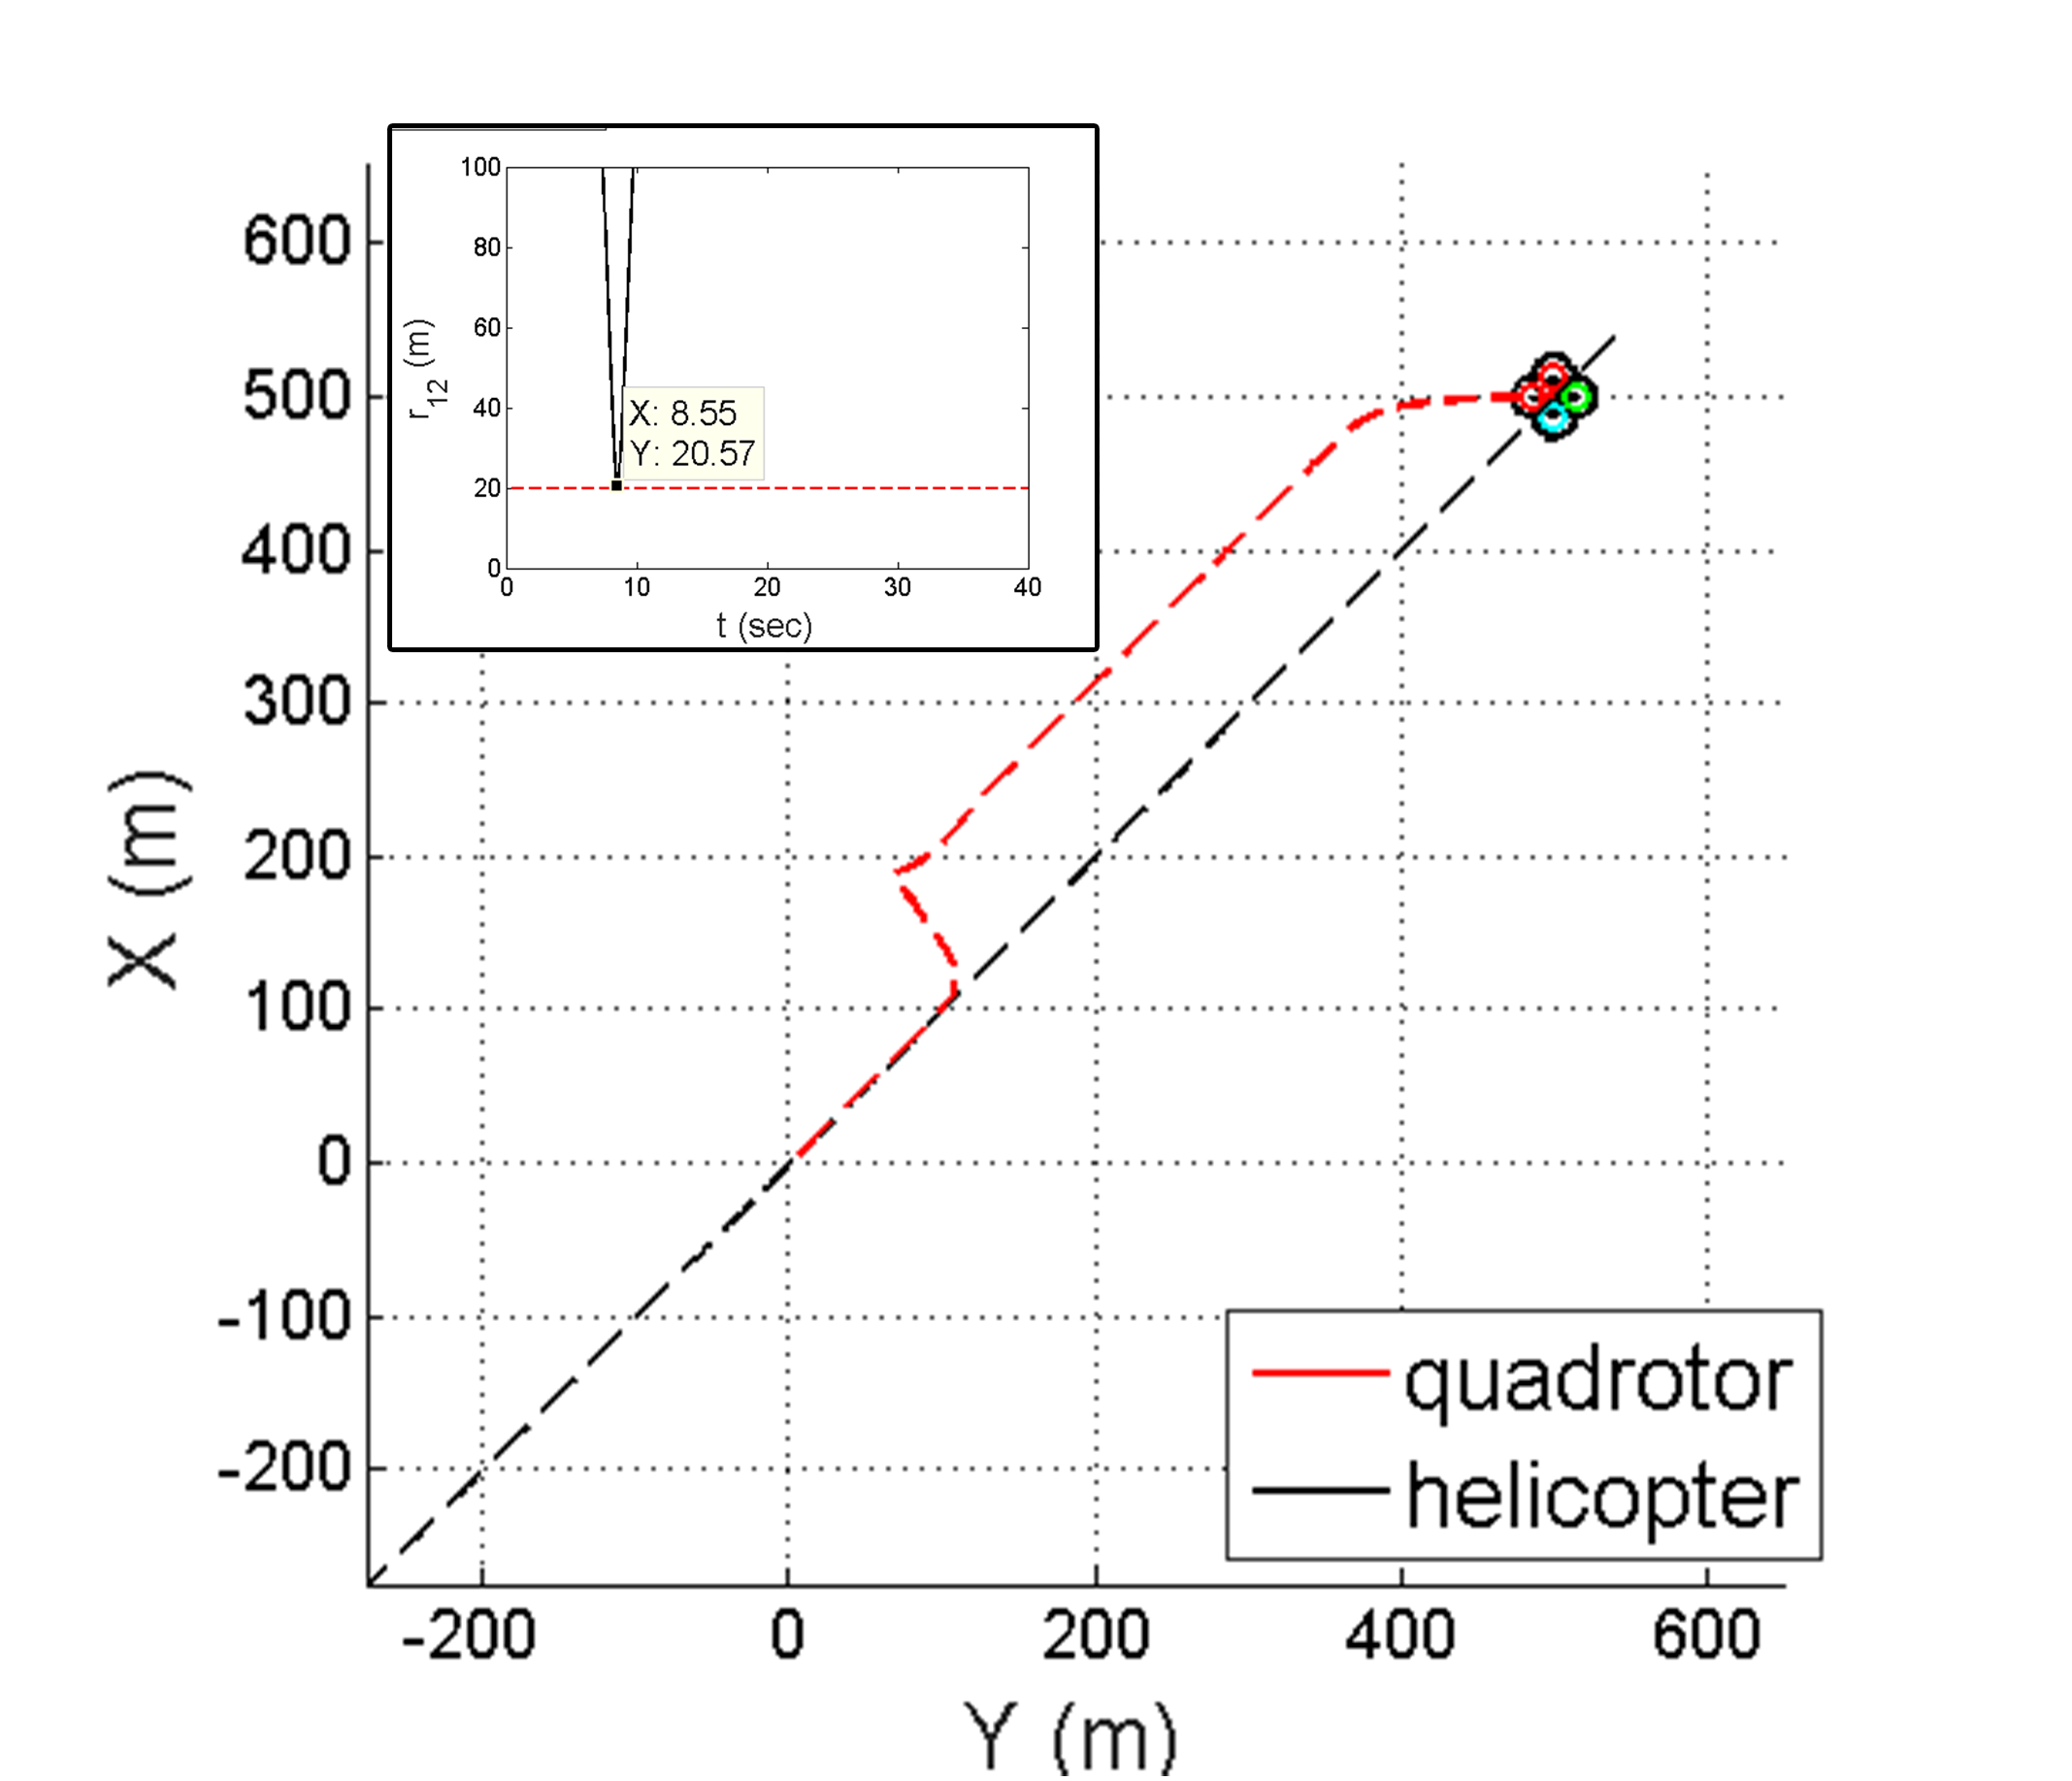
\includegraphics[width=\columnwidth]{waypoint_avoidance_trajectory}
        \caption{horizontal position trajectory}
        \label{fig:waypoint_avoidance_trajectory}
    \end{subfigure}
	\hfill
    \begin{subfigure}[b]{0.45\columnwidth}
        \centering
        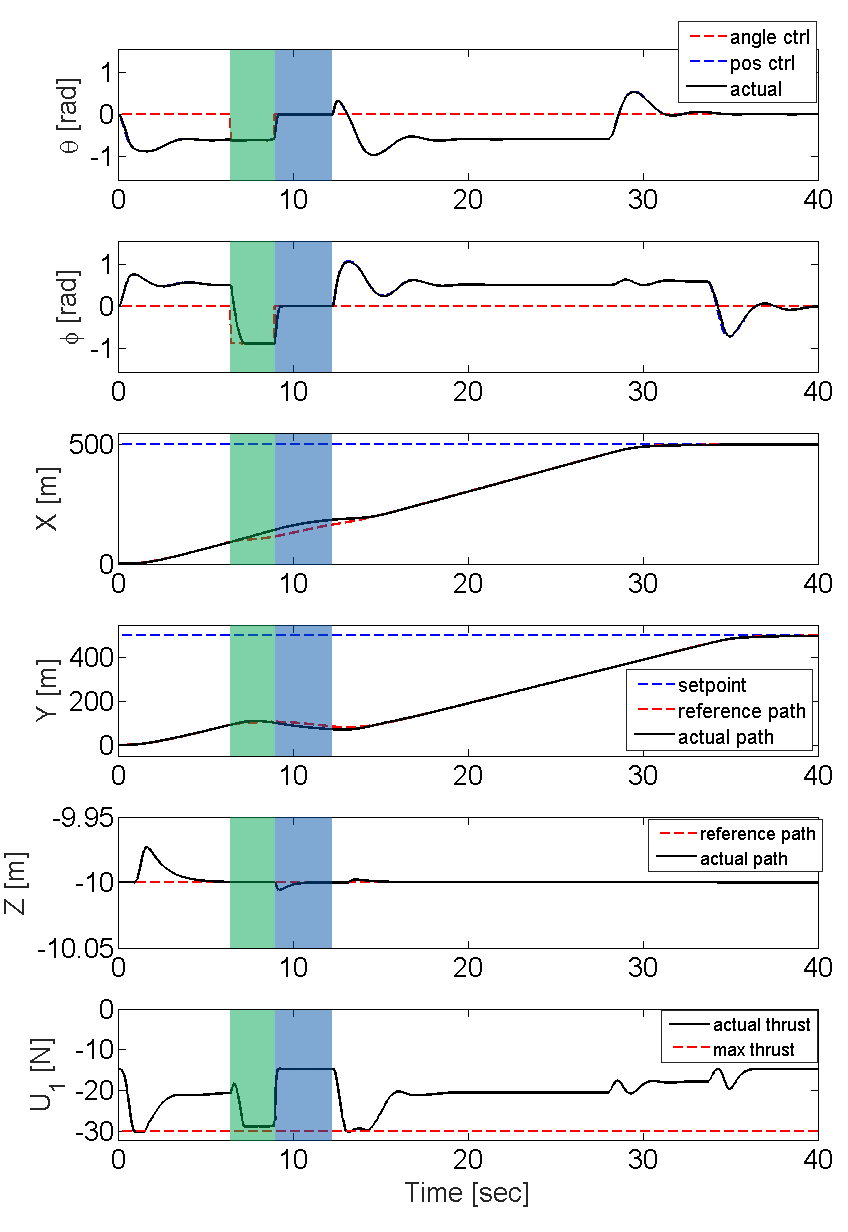
\includegraphics[width=\columnwidth]{waypoint_avoidance}
        \caption{time history of reference and control signals}
        \label{fig:waypoint_avoidance_signals}
    \end{subfigure}
    
    \caption{The quadrotor avoids a helicopter on the way to a destination. In (b), the green region indicates safety control is enabled, and the blue region is the stabilizing time after avoidance. Both the green and blue region uses angle control, and the white region uses position control.}
    \label{fig:waypoint_avoidance}
\end{figure}

%\begin{figure*}[!t]
%%\normalsize 		% ensure that we have normalsize text
%\begingroup\makeatletter\def\f@size{8}\check@mathfonts
%\begin{equation}
%\label{eq:state-space_expanded}
%\begin{split}
%\begin{bmatrix}
%\dot{X}\\ 
%\dot{Y}\\ 
%\dot{Z}\\ 
%\dot{\phi}\\ 
%\dot{\theta}\\ 
%\dot{\psi}\\ 
%\dot{V}_X\\ 
%\dot{V}_Y\\ 
%\dot{V}_Z\\ 
%\dot{\omega}_x\\ 
%\dot{\omega}_y\\ 
%\dot{\omega}_z
%\end{bmatrix}
%=
%\begin{bmatrix}
%V_X\\ 
%V_Y\\ 
%V_Z\\ 
%\omega_x+\omega_y sin\phi tan\theta+\omega_z cos\phi tan\theta\\ 
%\omega_ycos\phi-\omega_z sin\phi\\ 
%-\frac{c_t}{m}V_X\\ 
%-\frac{c_t}{m}V_Y\\ 
%-\frac{c_t}{m}V_Z\\ 
%\frac{I_y-I_z}{I_x}\omega_y \omega_z - \frac{c_r}{I_x}\omega_x^2-\frac{I_r}{I_x} \Omega\omega_y \\
%\frac{I_z-I_x}{I_y}\omega_x \omega_z - \frac{c_r}{I_y}\omega_y^2-\frac{I_r}{I_y} \Omega\omega_x \\ 
%\frac{I_x-I_y}{I_x}\omega_x \omega_y - \frac{c_r}{I_z}\omega_z^2 \\ 
%\end{bmatrix}
%+
%\begin{bmatrix}
%0 \\0 \\ 0\\ 0\\ 0\\ 0\\ 
%\frac{cos\phi sin\theta cos\psi + sin\phi sin\psi}{m} \\ 
%\frac{cos\phi sin\theta sin\psi - sin\phi cos\psi}{m} \\ 
%\frac{cos\phi cos\theta}{m} \\ 
%0 \\0 \\ 0
%\end{bmatrix}
%U_1+
%\begin{bmatrix}
%0\\ 0\\ 0\\ 0\\ 0\\ 0\\ 0\\ 0\\ 0\\ \frac{l}{I_x}\\ 0\\ 0
%\end{bmatrix}
%U_2+
%\begin{bmatrix}
%0\\ 0\\ 0\\ 0\\ 0\\ 0\\ 0\\ 0\\ 0\\ 0\\ \frac{l}{I_y}\\ 0
%\end{bmatrix}
%U_3+
%\begin{bmatrix}
%0\\ 0\\ 0\\ 0\\ 0\\ 0\\ 0\\ 0\\ 0\\ 0\\ 0\\ \frac{1}{I_z}
%\end{bmatrix}
%U_4
%\end{split}
%\end{equation}
%\endgroup
%\end{figure*}

\section{\textbf{Conclusion}}

In this paper, a hybrid controller with collision avoidance capability is presented in the context of high-speed heterogeneous flights. A concise position controller is formulated by adopting DSC techniques. In addition, a computationally feasible 2D optimal safety controller minimizing the avoidance duration is modified to be suitable for a 3D quadrotor model with rotational inertia. The combined hybrid controller is capable of performing optimal avoidance when flying to a destination autonomously. 

Some future work remains. First, the safety controller is implemented analytically in this paper, but it is possible to numerically evaluate the avoid set using the level-set toolbox. Then, a more sophisticated 2D model could be deployed. Second, the safety controller should be improved to handle a small multi-helicopter avoidance scenario. Third, the hybrid controller should be integrated with an air highway system, which is necessary to avoid multi-drone-to-drone collision. Lastly, a hardware implementation is necessary to confirm its effectiveness in real life.

%\appendices
%\section*{Appendix}
%
%Figure \ref{fig:backward_dynamics} shows the trajectory from $\left( x_{12}(t_0) , y_{12}(t_0) \right)$ to $\left( x_{12}(0) , y_{12}(0) \right)$. Decompose the trajectory along and perpendicular to the direction of $\theta_1^*$ into $d_1$ and $d_2$. Given the initial speed $v_i = v_{12}(t_0)sin\theta_1^*$, final speed $v_f = 0$, and the constant external force $-ma_{max}$, we have 
%
%\begin{equation*}
%\label{eq:derivation1}
%\begin{split}
%d_1 &= \frac{\left(v_{12}(t_0)sin\theta_1^*\right)^2}{2a_{max}} \\
%d_2 &= \left(v_{12}(t_0)cos\theta_1^*\right) \left( \frac{v_{12}(t_0)sin\theta_1^*}{2a_{max}} \right) \\
%\end{split}
%\end{equation*}
%
%Lastly, by geometry,
%
%\begin{equation*}
%\label{eq:derivation2}
%\begin{split}
%x_{12}(t_0) - d_1 cos\theta_1^* + d_2 sin\theta_1^* &= r_{min}cos\theta_1^* \\
%y_{12}(t_0) - d_1 sin\theta_1^* - d_2 cos\theta_1^* &= r_{min}sin\theta_1^* \\
%\end{split}
%\end{equation*}
%
%which results in (\ref{eq:backward_dyn}).
%
%
%\begin{figure}
%\centering
%\includegraphics[width=2.5in]{backward_dynamics}
%\caption{Backward dynamics diagram.}
%\label{fig:backward_dynamics}
%\end{figure}


%\begin{figure*}
%    \centering
%    \begin{subfigure}[b]{0.475\textwidth}
%        \centering
%        \includegraphics[width=\textwidth]{chattering_SM}
%        \caption[]%
%        {{sliding mode}}    
%        \label{fig:sliding_mode}
%    \end{subfigure}
%    \hfill
%    \begin{subfigure}[b]{0.475\textwidth}  
%        \centering 
%        \includegraphics[width=\textwidth]{tracking_SM_sat_smooth}
%        \caption[]%
%        {{sliding with saturation smoothing}}    
%        \label{fig:sliding_sat}
%    \end{subfigure}
%    \vskip\baselineskip
%    \begin{subfigure}[b]{0.475\textwidth}   
%        \centering 
%        \includegraphics[width=\textwidth]{tracking_SM_exp_smooth}
%        \caption[]%
%        {{sliding with logistical smoothing}}    
%        \label{fig:sliding_exp}
%    \end{subfigure}
%    \quad
%    \begin{subfigure}[b]{0.475\textwidth}   
%        \centering 
%        \includegraphics[width=\textwidth]{tracking_SM_linear_smooth}
%        \caption[]%
%        {{sliding with linear smoothing}}    
%        \label{fig:sliding_linear}
%    \end{subfigure}
%    \caption[]
%    {Comparison of tracking performance for different sliding controllers.} 
%    \label{fig:sliding_comparison}
%\end{figure*}



\bibliography{references}
\bibliographystyle{IEEEtran}

\end{document}

%%%%%%%%%%%%%%%%%%
% Latex references
%%%%%%%%%%%%%%%%%%

% \begin{figure}
% \centering
% \includegraphics[width=3.0in]{electro_thermal_model}
% \caption{The five-state electro-thermal model.}
% \label{electro_thermal_model}
% \end{figure}

% \begin{figure}
%   \centering
%     \begin{subfigure}[b]{0.3\textwidth}
%       \includegraphics[width=3.0in]{5state_coupled_noNoise}
%       \label{5state_coupled_noNoise}
%     \end{subfigure}%
%     \begin{subfigure}[b]{0.3\textwidth}
%       \includegraphics[width=3.0in]{5state_coupled_noise}
%       \label{5state_coupled_noise}
%     \end{subfigure}
%   \caption{Five-state parameter-coupled model results. }
%   \label{5state_coupled}
% \end{figure}

% \begin{itemize}
% \item \textbf{ITEM : } DESCRIPTION
% \end{itemize}

% \begin{enumerate}
% \item \textit{ASCEND\_START} -  Start gradient ascend
% \item \textit{DESCEND\_START} -  Start gradient descend
% \item \textit{TRANSMIT\_START} -  Start transmission of bot
% \item \textit{ARRIVAL} -  Ascending bot signals arrival to sentry bot
% \item \textit{ACK} -  Acknowledges receipt of above commands
% \item \textit{STOP\_ACK} -  Stops acknowledgement packet
% \end{enumerate}
